\section{Rate-Distorsion Curve}
\subsection{RD Curve for No Transformation}
Another important metric that many people use in image processing is the Rate-Distortion curve. This relates the entropy of an image at a particular $Q_{step}$ to the PSNR. Here I considered $Q_{step} \in [2, 4, 8, 16, 32, 64, 128]$ with no transformation the results of which are shown in Figure \ref{fig:RDNoTransform}.
\begin{figure}[H]
    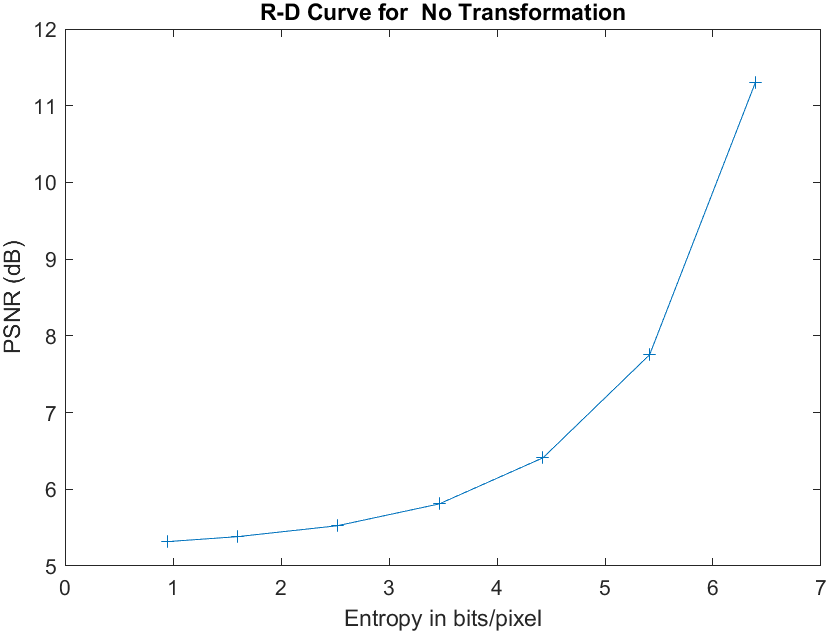
\includegraphics[width=0.8\textwidth]{RDNoTransform.png}
    \centering
    \caption{Rate-Distorsion Curve for No Transform}
    \label{fig:RDNoTransform}
\end{figure}

\subsection{RD Curve with Level 1 Haar}
Here I added data points for the level 1 Haar transform. 

\begin{figure}[H]
    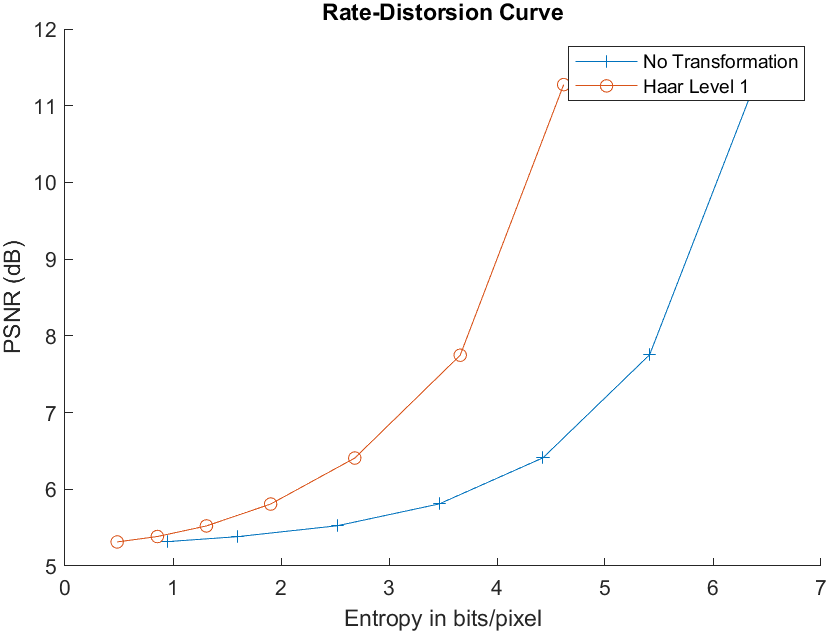
\includegraphics[width=0.8\textwidth]{RDWithTransform.png}
    \centering
    \caption{Rate-Distorsion Curve with Level 1 Haar}
    \label{fig:RDWithTransform}
\end{figure}

\subsection{Comparing Transform with No Transform}
Judging, by the PSNR value (high is better) we can clearly see that the Haar transform even at level 1 offers us lower bitrates at higher quality when compared with no transform at the same quantization level. This is ideal for sharing images over the internet where we want the highest quality for the lowest bitrate.